\subsection{Corriente Alterna}
\label{sec:corriente-alterna}

\subsubsection{Voltaje en corriente alterna}
\label{sec:voltaje-en-ca}

La corriente alterna debe su nombre a que la señal de voltaje tiene forma de una onda senoidal, a lo largo de la cual la magnitud del voltaje cambia continuamente, tal como vemos en la Figura \ref{fig:senoidal-voltaje}. El eje central representa el voltaje instantáneo con magnitud $0$, por lo cual los valores por debajo de este eje representan magnitudes con una polaridad negativa y los valores por encima del eje representan polaridad positiva. Véase que por cada $\pi$ radianes hay un cambio de ciclo, es decir termina un periodo.

\begin{figure}[h!]
    \centering
    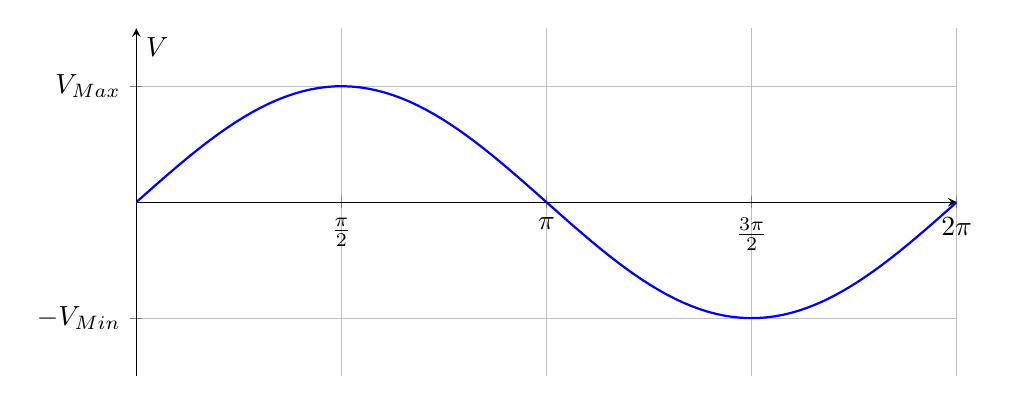
\begin{tikzpicture}
        \begin{axis}[
            domain=0:2*pi,
            samples=100,
            axis lines=middle,
            %xlabel=$t$,
            ylabel=$V$,
            xtick={0, pi/2, pi, 3*pi/2, 2*pi},
            xticklabels={$0$, $\frac{\pi}{2}$, $\pi$, $\frac{3\pi}{2}$, $2\pi$},
            ytick={-1, 0, 1},
            yticklabels={$-V_{Min}$, 0 , $V_{Max}$},
            ymin=-1.5,
            ymax=1.5,
            grid=major,
            width=12cm,
            height=6cm
        ]
        \addplot[blue, thick] {sin(deg(x))};
        \end{axis}
    \end{tikzpicture}
    \caption{Onda senoidal de voltaje}
    \label{fig:senoidal-voltaje}
\end{figure}

De modo que el voltaje instantáneo en cualquier punto de la onda es:

\[
  \upsilon = V_{M} \cdotp sen(\theta)
\]

donde:\\
\(\upsilon\) = Voltaje instantáneo\\
\(V_M\) = Voltaje máximo en Volts \\
\(\theta\) = Ángulo de giro (del generador)

\subsubsection{Intensidad de la corriente alterna}
\label{sec:intensidad-en-ca}

Cuando se conecta una carga a una linea de voltaje de corriente alterna, la intensidad de la corriente adquiere la misma forma senoidal (ver Figura \ref{fig:senoidal-corriente}).

\begin{figure}[h!]
    \centering
    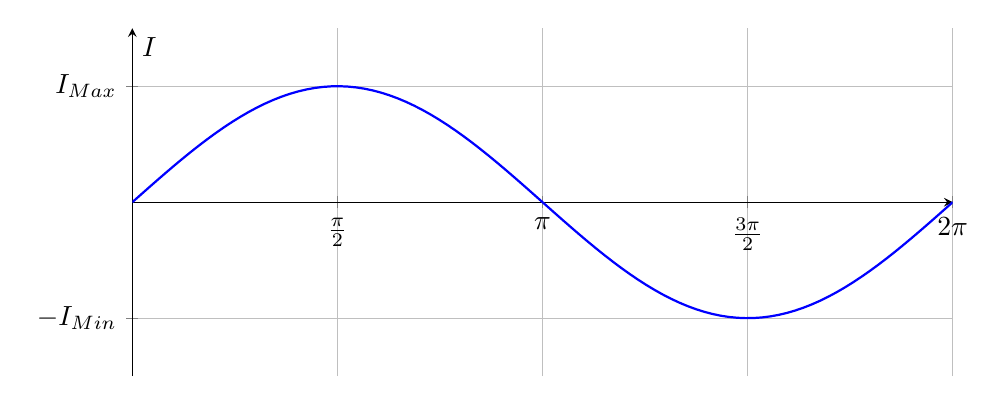
\begin{tikzpicture}
        \begin{axis}[
            domain=0:2*pi,
            samples=100,
            axis lines=middle,
            %xlabel=$t$,
            ylabel=$I$,
            xtick={0, pi/2, pi, 3*pi/2, 2*pi},
            xticklabels={$0$, $\frac{\pi}{2}$, $\pi$, $\frac{3\pi}{2}$, $2\pi$},
            ytick={-1, 0, 1},
            yticklabels={$-I_{Min}$, 0 , $I_{Max}$},
            ymin=-1.5,
            ymax=1.5,
            grid=major,
            width=12cm,
            height=6cm
        ]
        \addplot[blue, thick] {sin(deg(x))};
        \end{axis}
    \end{tikzpicture}
    \caption{Onda senoidal de intensidad de corriente}
    \label{fig:senoidal-corriente}
\end{figure}

De la ley de Ohm, $V = R \cdotp I$, podemos obtener que el valor máximo de la corriente se puede calcular de la forma:

\[
  I = \frac{V_{M} }{R}
\]

donde:\\
\(I\) = Intensidad máxima\\
\(V_M\) = Voltaje máximo en Volts \\
\(R\) = Resistencia equivalente a la carga

Y del mismo modo que sucede con el voltaje se puede obtener la magnitud de la intensidad de la corriente en cualquier punto utilizando la función:


\subsubsection{Potencia y consumo de energía en circuitos de CA}

\subsubsection{Técnicas para la medición de la intensidad de la corriente}

\subsection{Sensor ACS712}
\label{sec:sensor-acs712}

\subsection{Microcontrolador ESP32}
\label{sec:micr-esp32}

\subsection{Regla compuesta de Simpson}
\label{sec:regla-compuesta-de}

\subsubsection{Aplicación de la regla de Simpson para cálcular el consumo de energía eléctrica}
